\section{Transition-based Dependency Parsing}
A transition-based parser frames the problem of parsing as a series of action~(shift/reduce) decisions given a configuration. Dependency parsing is an NLP parsing problem where the objective is to obtain a grammatical structure in the form of a parse tree. A parse tree contains directed edges going from a source~(or, head) token to a target~(or, dependent) token. Each edge is labeled with a dependency relation from a fixed set of relations. As an example, Figure \ref{fig:ex} shows a dependency parse tree for the sentence ``Mary lives in California''.
\begin{figure}[h!]
    \centering
    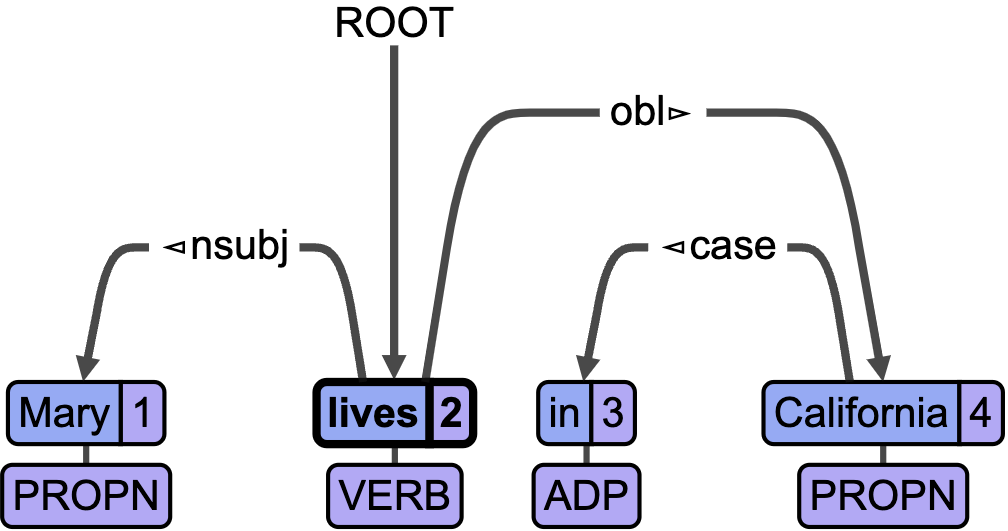
\includegraphics[width=0.4\textwidth]{ud_example.png}
    \caption{An example dependency parse tree for the sentence ``Mary lives in California''.}
    \label{fig:ex}
\end{figure}

The configuration of a transition-based parser is also known as a parse state.  Transition-based dependency parser's parse state comprises of three components -- the stack, the buffer, and a set of dependencies. Initially, the stack and the set of dependencies are empty, while the buffer is initialized by the set of tokens in the sentence. Given a parse state, the best possible action needs to be predicted to update the parse state. There are three types of actions possible-
\begin{enumerate}
    \item \textbf{Shift}: This moves the next element in the buffer to the top of the stack. Consequently, the stack and the buffer are changed in the parse state.
    \item \textbf{ReduceLeft$_{r}$ or LeftArc$_{r}$}: This takes the top two elements of the stack. A dependency with relation \emph{r} between the elements is added such that the topmost element of the stack is the head. The second element from the top of the stack is removed.  Consequently, the stack and the set of dependencies are changed in the parse state.
    \item \textbf{ReduceRight$_{r}$ or RightArc$_{r}$}: This takes the top two elements of the stack. A dependency with relation \emph{r} between the elements is added such that the second element from the top of the stack is the head. The topmost element of the stack is removed.  Consequently, the stack and the set of dependencies are changed in the parse state.
\end{enumerate}
Action decisions are made till the stack and the buffer are empty. This configuration is known as the final state. At this point, the set of dependencies corresponds to the dependency parse of the sentence. See the lecture notes for a worked-out example.

Note that we haven't mentioned how the actions are decided. This is, typically, done using a multi-class classifier which takes a representation of the parse state as input and produces an action decision.

\paragraph{Evaluation.} Dependency parsers are evaluated using two metrics-- Unlabeled Attachment Score~(UAS), and Labeled Attachment Score~(LAS). UAS is the proportion of dependents that were assigned the correct head. LAS is the proportion of dependents that were assigned the correct head with the correct dependency relation label. Intuitively, LAS has to be less than or equal to UAS. 